\documentclass[../main.tex]{subfiles}


\begin{document}
\raggedright

To begin with, the extenuating circumstances page\cite{ecfuni} would need to have a link to the portal which will contain a login page allowing the student to login with his or her university email. Once the student has logged in, an option to start a new extenuating circumstance form will be displayed and clicking on that the student will be presented with a form to fill online. On successful completion of the online form, the data will be stored on their profile and displayed on the "Dashboard" of the portal. The same form can then be accessed over time with new feedback, approval and other statuses. Any updates by the scrutiny committee will be notified to the student via the secretary and the portal. \\[4mm]

The portal would also allow the scrutiny committee to login and control the movement of the forms as well as provide feedback and comments to the student regarding their circumstance. They would also be able to request more proof and evidence if need be. The forms can then be processed further and exported as documents such as PDF's and TXT's allowing the relevant stakeholder to print or share. Figure~\ref{fig:portal1} describes the authentication and users process. In this case the secretary is part of the scrutiny committee. 

	\begin{figure}[H]
        \center{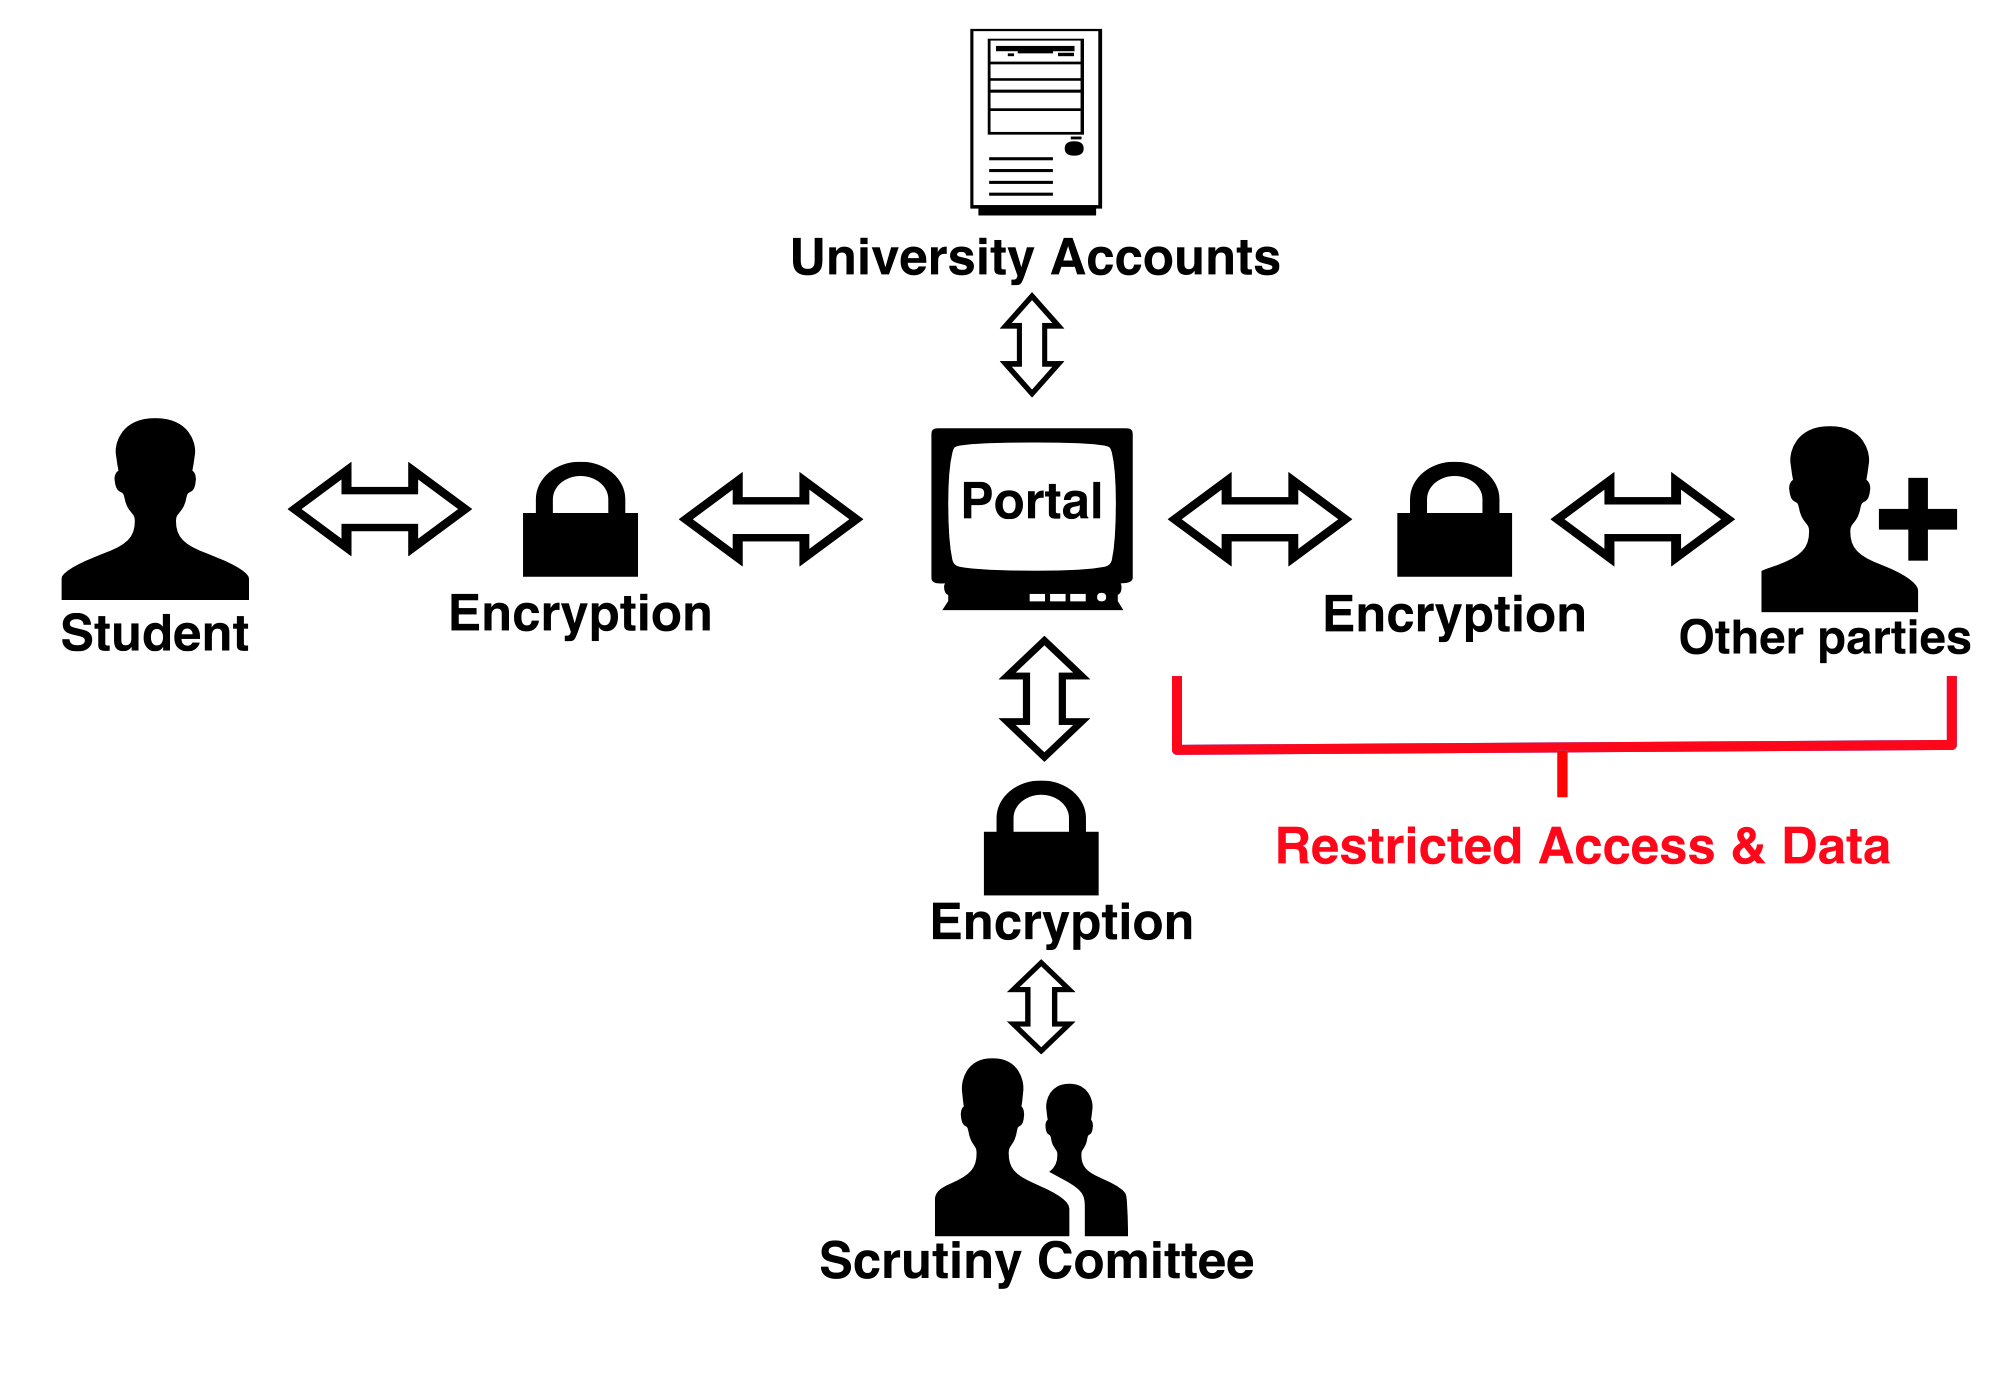
\includegraphics[scale=0.3]
        {images/portal1.png}}
        \caption{\label{fig:portal1} Portal and users.}
      \end{figure}

The web system will be entirely encrypted and data will be stored in a secure database as presented earlier in Figure~\ref{fig:basicwebdesign}. This allows total security of the information stored and only users with access will be allowed to get that information. Some users will be restricted such as the other parties who get the students condition without knowing exactly what it is they are having trouble with. This allows confidentiality while allowing access at the same time. \\[4mm]

If the system is able to complete all the above steps and keep the security intact then we will have been able to successfully achieve the requirements for this project. In order to successfully evaluate the project, each of the requirements will need to be described with the implementation and if it was fulfilled successfully. 

\end{document}
